\documentclass[11pt,a4paper]{article}

% Packages
\usepackage[utf8]{inputenc}
\usepackage[T1]{fontenc}
\usepackage{geometry}
\usepackage{graphicx}
\usepackage{amsmath}
\usepackage{amssymb}
\usepackage{listings}
\usepackage{xcolor}
\usepackage{hyperref}
\usepackage{booktabs}
\usepackage{longtable}
\usepackage{fancyhdr}
\usepackage{titlesec}
\usepackage{caption}
\usepackage{float}
\usepackage{enumitem}
\usepackage{tikz}
\usetikzlibrary{shapes,arrows,positioning,fit,backgrounds}

% Page geometry
\geometry{margin=2.5cm}

% Code listing style
\definecolor{codegreen}{rgb}{0,0.6,0}
\definecolor{codegray}{rgb}{0.5,0.5,0.5}
\definecolor{codepurple}{rgb}{0.58,0,0.82}
\definecolor{backcolour}{rgb}{0.95,0.95,0.92}

\lstdefinestyle{mystyle}{
    backgroundcolor=\color{backcolour},
    commentstyle=\color{codegreen},
    keywordstyle=\color{blue},
    numberstyle=\tiny\color{codegray},
    stringstyle=\color{codepurple},
    basicstyle=\ttfamily\footnotesize,
    breakatwhitespace=false,
    breaklines=true,
    captionpos=b,
    keepspaces=true,
    numbers=left,
    numbersep=5pt,
    showspaces=false,
    showstringspaces=false,
    showtabs=false,
    tabsize=2,
    frame=single
}
\lstset{style=mystyle}

% Hyperref setup
\hypersetup{
    colorlinks=true,
    linkcolor=blue,
    filecolor=magenta,
    urlcolor=cyan,
    pdftitle={SRT Drive Controller Technical Documentation},
    pdfauthor={Acre Road Observatory}
}

% Header and footer
\pagestyle{fancy}
\fancyhf{}
\fancyhead[L]{SRT Drive Controller}
\fancyhead[R]{Technical Documentation}
\fancyfoot[C]{\thepage}

% Title
\title{
    \vspace{-1cm}
    \textbf{Small Radio Telescope Drive Controller} \\
    \Large Technical Documentation and Operations Manual \\
    \vspace{0.5cm}
    \large Version 1.1
}
\author{
    Acre Road Observatory \\
    University of Glasgow
}
\date{March 2026}

\begin{document}

\maketitle

\begin{abstract}
This document provides comprehensive technical documentation for the Small Radio Telescope (SRT) Drive Controller system designed for 21\,cm hydrogen line observations at Acre Road Observatory, Glasgow. The system comprises a multi-layered architecture incorporating an Arduino Due microcontroller for low-level motor control, an ESP32-S3 for network interface and coordinate transformations, and a GNU Radio-based receiver with web scheduling capabilities. This document details the hardware configuration, software architecture, communication protocols, coordinate transformation algorithms, installation procedures, and operational guidelines necessary for the deployment and maintenance of the telescope control system.
\end{abstract}

\tableofcontents
\newpage

%==============================================================================
\section{Introduction}
%==============================================================================

\subsection{Purpose and Scope}

The SRT Drive Controller is a complete control system for an alt-azimuth mounted radio telescope operating at 1420.405\,MHz (the hydrogen line). The system enables both manual and automated observations, supporting:

\begin{itemize}
    \item Real-time telescope positioning via web interface
    \item Integration with planetarium software (Stellarium)
    \item Automated coordinate conversion from celestial to horizontal coordinates
    \item Scheduled observations with data acquisition
    \item Sun and Moon tracking capabilities
\end{itemize}

\subsection{System Overview}

The telescope control system employs a layered architecture separating concerns across multiple processing units:

\begin{enumerate}
    \item \textbf{Arduino Due} --- Low-level motor control, position encoding, limit switch monitoring, and current sensing
    \item \textbf{ESP32-S3} --- Network interface, astronomical coordinate transformations, web server, and Stellarium protocol implementation
    \item \textbf{H1 Receiver} --- GNU Radio-based spectrum analyser for 21\,cm data acquisition
    \item \textbf{Observation Scheduler} --- Web-based automation coordinating telescope pointing and data recording
\end{enumerate}

\subsection{Document Organisation}

This document is organised as follows: Section~\ref{sec:architecture} presents the system architecture; Section~\ref{sec:hardware} details the hardware components; Section~\ref{sec:due-firmware} describes the Arduino Due firmware; Section~\ref{sec:esp32} covers the ESP32 controller; Section~\ref{sec:coordinates} explains the coordinate transformation algorithms; Section~\ref{sec:receiver} describes the receiver and scheduler; Section~\ref{sec:installation} provides installation procedures; Section~\ref{sec:operation} covers operational procedures; and Section~\ref{sec:troubleshooting} addresses common issues.

%==============================================================================
\section{System Architecture}
\label{sec:architecture}
%==============================================================================

\subsection{Architectural Overview}

The system architecture follows a hierarchical design principle, with each layer responsible for specific functionality. Figure~\ref{fig:architecture} illustrates the component relationships and communication paths.

\begin{figure}[H]
\centering
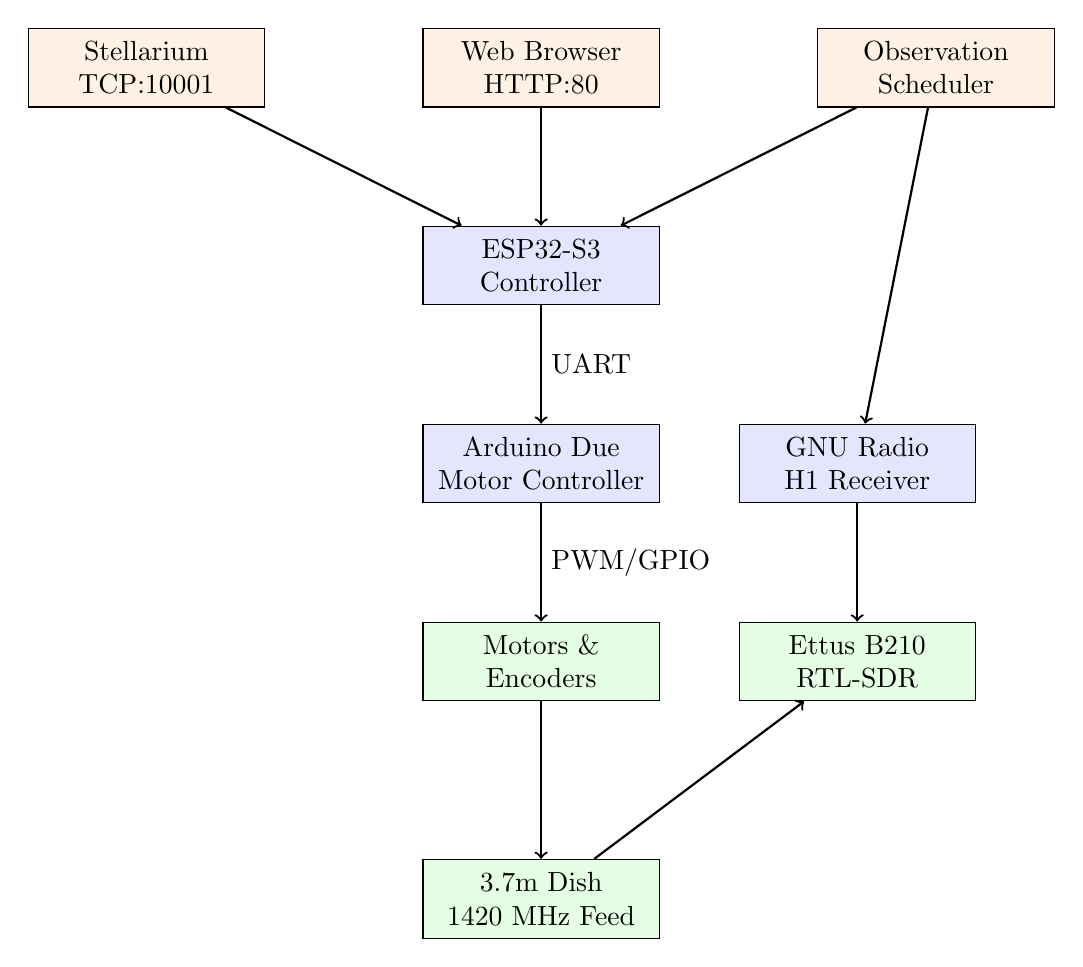
\begin{tikzpicture}[
    node distance=1.5cm,
    box/.style={rectangle, draw, minimum width=3cm, minimum height=1cm, align=center, fill=blue!10},
    hwbox/.style={rectangle, draw, minimum width=3cm, minimum height=1cm, align=center, fill=green!10},
    extbox/.style={rectangle, draw, minimum width=3cm, minimum height=1cm, align=center, fill=orange!10},
    arrow/.style={->, thick}
]

% External systems
\node[extbox] (stellarium) {Stellarium\\TCP:10001};
\node[extbox, right=2cm of stellarium] (browser) {Web Browser\\HTTP:80};
\node[extbox, right=2cm of browser] (scheduler) {Observation\\Scheduler};

% ESP32
\node[box, below=1.5cm of browser] (esp32) {ESP32-S3\\Controller};

% Arduino Due
\node[box, below=1.5cm of esp32] (due) {Arduino Due\\Motor Controller};

% Hardware
\node[hwbox, below=1.5cm of due] (motors) {Motors \&\\Encoders};

% Receiver
\node[box, right=1cm of due] (receiver) {GNU Radio\\H1 Receiver};

% SDR
\node[hwbox, below=1.5cm of receiver] (sdr) {Ettus B210\\RTL-SDR};

% Antenna
\node[hwbox, below=2cm of motors] (antenna) {3.7m Dish\\1420 MHz Feed};

% Connections
\draw[arrow] (stellarium) -- (esp32);
\draw[arrow] (browser) -- (esp32);
\draw[arrow] (scheduler) -- (esp32);
\draw[arrow] (scheduler) -- (receiver);
\draw[arrow] (esp32) -- node[right] {UART} (due);
\draw[arrow] (due) -- node[right] {PWM/GPIO} (motors);
\draw[arrow] (receiver) -- (sdr);
\draw[arrow] (antenna) -- (sdr);
\draw[arrow] (motors) -- (antenna);

\end{tikzpicture}
\caption{System architecture showing component relationships and communication interfaces}
\label{fig:architecture}
\end{figure}

\subsection{Data Flow}

The primary data flow for a typical observation proceeds as follows:

\begin{enumerate}
    \item User or scheduler specifies target coordinates (RA/Dec, Galactic, or direct Alt/Az)
    \item ESP32 converts celestial coordinates to horizontal (Alt/Az) using current sidereal time
    \item ESP32 transmits target position to Arduino Due via UART
    \item Arduino Due calculates motion profile and drives motors with PWM
    \item Reed switch encoders provide position feedback
    \item Due reports position and status to ESP32
    \item ESP32 updates web interface and Stellarium position
    \item Receiver captures spectrum data once telescope is on target
\end{enumerate}

\subsection{Communication Interfaces}

Table~\ref{tab:interfaces} summarises the communication interfaces employed throughout the system.

\begin{table}[H]
\centering
\caption{System communication interfaces}
\label{tab:interfaces}
\begin{tabular}{llll}
\toprule
\textbf{Interface} & \textbf{Protocol} & \textbf{Speed} & \textbf{Purpose} \\
\midrule
Due $\leftrightarrow$ ESP32 & UART Serial & 115200 baud & Position commands, status \\
ESP32 $\leftrightarrow$ Browser & HTTP & TCP:80 & Web interface, API \\
ESP32 $\leftrightarrow$ Stellarium & TCP & Port 10001 & Telescope protocol \\
Due $\leftrightarrow$ USB & Serial & 115200 baud & Debug, direct control \\
ESP32 WiFi & IEEE 802.11 & --- & Network connectivity \\
ESP32 Ethernet & 10/100 Mbps & W5500 SPI & Wired network \\
\bottomrule
\end{tabular}
\end{table}

%==============================================================================
\section{Hardware Configuration}
\label{sec:hardware}
%==============================================================================

\subsection{Arduino Due Microcontroller}

The Arduino Due serves as the real-time motor control platform, selected for its:

\begin{itemize}
    \item ARM Cortex-M3 processor (84\,MHz) with deterministic interrupt handling
    \item 12-bit analogue-to-digital converters for current sensing
    \item Multiple hardware UART interfaces
    \item PWM outputs with adequate resolution for smooth motor control
    \item 3.3\,V logic levels compatible with the ESP32
\end{itemize}

\subsubsection{Pin Assignments}

Table~\ref{tab:due-pins} details the complete pin assignment for the Arduino Due.

\begin{table}[H]
\centering
\caption{Arduino Due pin assignments}
\label{tab:due-pins}
\begin{tabular}{llll}
\toprule
\textbf{Function} & \textbf{Pin} & \textbf{Wire Colour} & \textbf{Notes} \\
\midrule
\multicolumn{4}{l}{\textit{Fault Flags (inputs)}} \\
Az Fault Flag 1 & 5 & Blue & Motor driver status \\
Az Fault Flag 2 & 4 & Purple & Motor driver status \\
Alt Fault Flag 1 & 7 & Blue & Motor driver status \\
Alt Fault Flag 2 & 6 & Purple & Motor driver status \\
\midrule
\multicolumn{4}{l}{\textit{Motor Control (outputs)}} \\
Az PWM & 8 & Green & Speed control (inverted) \\
Az Direction & 9 & Yellow & LOW=West, HIGH=East \\
Alt PWM & 10 & Green & Speed control (inverted) \\
Alt Direction & 11 & Yellow & LOW=Down, HIGH=Up \\
\midrule
\multicolumn{4}{l}{\textit{Driver Reset (outputs)}} \\
Az Reset & 22 & Black & HIGH=enabled \\
Alt Reset & 24 & White & HIGH=enabled \\
\midrule
\multicolumn{4}{l}{\textit{Position Encoders (inputs)}} \\
Az Pulses & 12 & Blue & Reed switch, falling edge \\
Alt Pulses & 13 & Orange & Reed switch, falling edge \\
\midrule
\multicolumn{4}{l}{\textit{Current Sensors (analogue inputs)}} \\
Az Current & A1 & Black & ACS712 hall-effect \\
Alt Current & A0 & White & ACS712 hall-effect \\
\midrule
\multicolumn{4}{l}{\textit{Serial1 (ESP32 interface)}} \\
TX1 & 18 & --- & To ESP32 RX \\
RX1 & 19 & --- & From ESP32 TX \\
\bottomrule
\end{tabular}
\end{table}

\subsection{Motor Drive System}

\subsubsection{H-Bridge Motor Drivers}

The system employs H-bridge motor drivers with the following characteristics:

\begin{itemize}
    \item Dual fault flag outputs (FF1, FF2) indicating:
    \begin{itemize}
        \item FF1=LOW, FF2=HIGH: Short circuit
        \item FF1=HIGH, FF2=LOW: Overheating
        \item FF1=HIGH, FF2=HIGH: Undervoltage
    \end{itemize}
    \item Active-low reset input
    \item PWM speed control with inverted logic (255 = stopped, 0 = full speed)
    \item Direction control input
\end{itemize}

\subsubsection{Position Encoders}

Position feedback is provided by reed switch encoders mounted on each axis:

\begin{itemize}
    \item Resolution: 2 pulses per degree (0.5$^\circ$ positioning accuracy)
    \item Detection: Falling edge triggered interrupts
    \item Debouncing: 15\,ms minimum interval between valid pulses
\end{itemize}

\subsubsection{Current Sensing}

Motor current is monitored using ACS712 hall-effect current sensors:

\begin{itemize}
    \item Zero-current output voltage: 2.5\,V
    \item Sensitivity: 66\,mV/A
    \item Default overcurrent threshold: 5.0\,A
\end{itemize}

The current reading is computed as:
\begin{equation}
I = \frac{V_{ADC} - V_{offset}}{S}
\end{equation}
where $V_{ADC}$ is the measured voltage, $V_{offset} = 2.5$\,V, and $S = 0.066$\,V/A.

\subsection{ESP32-S3 Controller}

The ESP32-S3 provides the network interface and computational resources for coordinate transformations:

\begin{itemize}
    \item Dual-core Xtensa LX7 processor
    \item WiFi 802.11 b/g/n (2.4\,GHz)
    \item 4\,MB flash, 512\,KB SRAM
    \item MicroPython runtime environment
\end{itemize}

\subsubsection{ESP32 to Arduino Due Wiring}

\begin{table}[H]
\centering
\caption{ESP32-S3 to Arduino Due serial connection}
\begin{tabular}{lll}
\toprule
\textbf{ESP32-S3} & \textbf{Arduino Due} & \textbf{Function} \\
\midrule
GPIO17 & Pin 19 (RX1) & ESP32 TX $\rightarrow$ Due RX \\
GPIO18 & Pin 18 (TX1) & ESP32 RX $\leftarrow$ Due TX \\
GND & GND & Common ground \\
\bottomrule
\end{tabular}
\end{table}

\subsubsection{W5500 Ethernet Module (Optional)}

For installations requiring wired network connectivity:

\begin{table}[H]
\centering
\caption{W5500 Ethernet module wiring}
\begin{tabular}{lll}
\toprule
\textbf{W5500} & \textbf{ESP32-S3} & \textbf{Function} \\
\midrule
MOSI & GPIO11 & SPI data out \\
MISO & GPIO13 & SPI data in \\
SCK & GPIO12 & SPI clock \\
CS & GPIO10 & Chip select \\
RST & GPIO9 & Reset \\
3.3V & 3.3V & Power \\
GND & GND & Ground \\
\bottomrule
\end{tabular}
\end{table}

\subsection{Operational Limits}

\begin{table}[H]
\centering
\caption{Telescope position limits}
\label{tab:limits}
\begin{tabular}{lll}
\toprule
\textbf{Axis} & \textbf{Minimum} & \textbf{Maximum} \\
\midrule
Altitude (hardware) & 0$^\circ$ (horizon) & 90$^\circ$ (zenith) \\
Altitude (software) & 0$^\circ$ & 90$^\circ$ \\
Azimuth (hardware) & 0$^\circ$ (North) & 355$^\circ$ \\
Azimuth (software) & 2$^\circ$ & 353$^\circ$ \\
\bottomrule
\end{tabular}
\end{table}

The two-tier limit system provides a 2$^\circ$ safety margin between software limits and physical stops.

%==============================================================================
\section{Arduino Due Firmware}
\label{sec:due-firmware}
%==============================================================================

\subsection{Firmware Overview}

The Arduino Due firmware (\texttt{src/main.cpp}) implements a state machine-based motor controller with the following responsibilities:

\begin{itemize}
    \item Automatic homing sequence on startup
    \item Smooth motion profiles with acceleration/deceleration ramps
    \item Position tracking via interrupt-driven encoder counting
    \item Safety monitoring (overcurrent, stall detection, limit switches)
    \item Serial command interface
    \item Configuration persistence to flash memory
\end{itemize}

\subsection{State Machine}

The controller operates as a finite state machine with five primary states:

\begin{figure}[H]
\centering
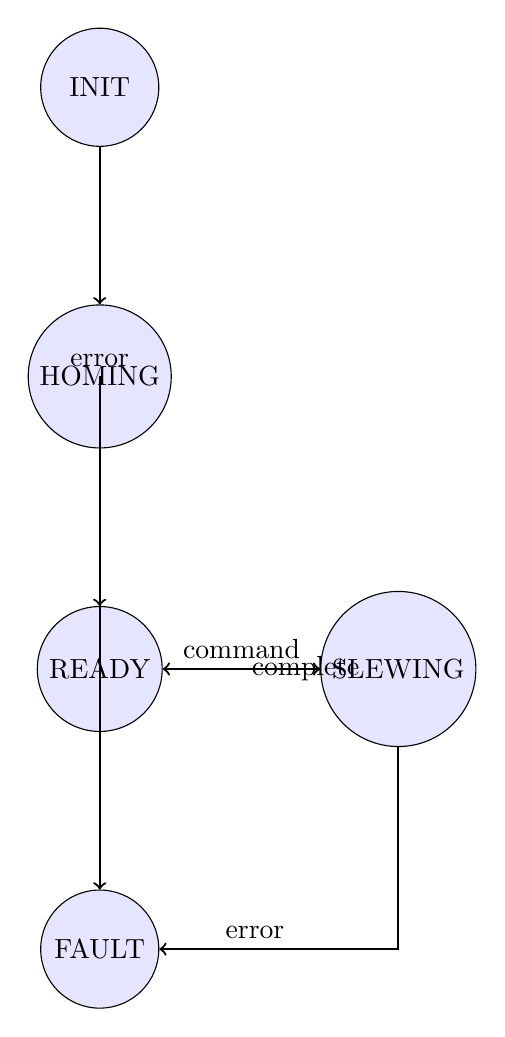
\begin{tikzpicture}[
    node distance=2cm,
    state/.style={circle, draw, minimum size=1.5cm, align=center, fill=blue!10},
    arrow/.style={->, thick}
]

\node[state] (init) {INIT};
\node[state, below=of init] (homing) {HOMING};
\node[state, below=of homing] (ready) {READY};
\node[state, right=of ready] (slewing) {SLEWING};
\node[state, below=of ready] (fault) {FAULT};

\draw[arrow] (init) -- (homing);
\draw[arrow] (homing) -- (ready);
\draw[arrow] (homing) -| node[above,pos=0.2] {error} (fault);
\draw[arrow] (ready) -- node[above] {command} (slewing);
\draw[arrow] (slewing) -- node[right] {complete} (ready);
\draw[arrow] (slewing) |- node[above,pos=0.8] {error} (fault);

\end{tikzpicture}
\caption{Controller state machine diagram}
\label{fig:state-machine}
\end{figure}

\begin{description}
    \item[INIT] Hardware initialisation, GPIO configuration, driver enabling
    \item[HOMING] Driving to limit switches, establishing position reference
    \item[READY] Idle state, accepting commands
    \item[SLEWING] Active motion toward target position
    \item[FAULT] Error condition, motors disabled
\end{description}

\subsection{Homing Sequence}

The homing procedure establishes the absolute position reference:

\begin{enumerate}
    \item Both motors drive toward their respective limit switches (azimuth west, altitude down)
    \item When no encoder pulses are received for 2 seconds (stall timeout), the motor is considered at the limit
    \item Position counters are reset to zero
    \item Motors drive to the home position (default: Alt=0$^\circ$, Az=180$^\circ$)
    \item System transitions to READY state
\end{enumerate}

\subsection{Motion Profiles}

Smooth motion profiles prevent structural oscillation and mechanical stress:

\subsubsection{Acceleration Ramp}

The PWM value ramps linearly from minimum speed to full speed over the configured ramp-up time (default 500\,ms):

\begin{equation}
PWM(t) = PWM_{min} + \frac{(PWM_{full} - PWM_{min}) \cdot t}{T_{ramp}}
\end{equation}

where $PWM_{min} = 220$ (minimum speed), $PWM_{full} = 0$ (full speed), and $T_{ramp}$ is the ramp-up time.

\subsubsection{Deceleration Ramp}

Deceleration uses a quadratic profile based on remaining distance to target (default 7$^\circ$):

\begin{equation}
PWM(d) = PWM_{full} + (PWM_{min} - PWM_{full}) \cdot \left(1 - \frac{d}{d_{ramp}}\right)^2
\end{equation}

where $d$ is the remaining distance and $d_{ramp}$ is the deceleration distance.

\subsection{Serial Command Interface}

The firmware accepts commands via USB serial (Programming Port) and Serial1 (ESP32 connection) at 115200 baud.

\subsubsection{Motion Commands}

\begin{table}[H]
\centering
\caption{Motion commands}
\begin{tabular}{ll}
\toprule
\textbf{Command} & \textbf{Description} \\
\midrule
\texttt{<alt> <az>} & Slew to position (e.g., \texttt{45.0 180.0}) \\
\texttt{DRIVE <alt> <az>} & Slew to position (explicit form) \\
\texttt{HOME} & Run homing sequence \\
\texttt{STOP} & Emergency stop \\
\texttt{RESET} & Clear fault and re-home \\
\bottomrule
\end{tabular}
\end{table}

\subsubsection{Configuration Commands}

\begin{table}[H]
\centering
\caption{Configuration commands}
\begin{tabular}{ll}
\toprule
\textbf{Command} & \textbf{Description} \\
\midrule
\texttt{STATUS} & Show current position and status \\
\texttt{CONFIG} & Show all configuration parameters \\
\texttt{SET <param> <value>} & Set configuration parameter \\
\texttt{SAVE} & Save configuration to flash \\
\texttt{LOAD} & Load configuration from flash \\
\texttt{DEFAULTS} & Reset to factory defaults \\
\texttt{HELP} & Show command help \\
\bottomrule
\end{tabular}
\end{table}

\subsubsection{Configurable Parameters}

\begin{table}[H]
\centering
\caption{SET command parameters}
\begin{tabular}{llll}
\toprule
\textbf{Parameter} & \textbf{Description} & \textbf{Default} & \textbf{Unit} \\
\midrule
ALTMIN & Altitude software minimum & 0 & degrees \\
ALTMAX & Altitude software maximum & 90 & degrees \\
AZMIN & Azimuth software minimum & 2 & degrees \\
AZMAX & Azimuth software maximum & 353 & degrees \\
HOMEALT & Home altitude position & 0 & degrees \\
HOMEAZ & Home azimuth position & 180 & degrees \\
RAMPUP & Acceleration time & 500 & ms \\
RAMPDOWN & Deceleration distance & 7 & degrees \\
STOPRAMP & Reversal deceleration time & 300 & ms \\
CURRENT & Overcurrent threshold & 5.0 & Amps \\
STALL & Stall detection timeout & 2000 & ms \\
\bottomrule
\end{tabular}
\end{table}

\subsection{Status Output Format}

The controller outputs status in a machine-parseable format:

\begin{lstlisting}[language=bash,caption={Status output examples}]
Alt:45.0 Az:180.0 Ialt:0.52A Iaz:0.38A Status:Ready
Alt:30.0 Az:150.0 Ialt:2.10A Iaz:1.85A Status:Slewing -> Alt:45.0 Az:180.0
Alt:30.0 Az:150.0 Ialt:5.20A Iaz:0.00A Status:FAULT [Altitude motor overcurrent]
\end{lstlisting}

\subsection{Fault Detection}

The system monitors multiple fault conditions:

\begin{table}[H]
\centering
\caption{Fault conditions and detection}
\begin{tabular}{lll}
\toprule
\textbf{Fault} & \textbf{Detection} & \textbf{Likely Cause} \\
\midrule
Short circuit & FF1=LOW, FF2=HIGH & Wiring fault, motor failure \\
Overheating & FF1=HIGH, FF2=LOW & Prolonged high current \\
Undervoltage & FF1=HIGH, FF2=HIGH & Power supply issue \\
Overcurrent & Current $>$ 5.0\,A & Obstruction, binding \\
Stall & No pulses for 2\,s & Motor failure, jam \\
Position bounds & Exceeds limits & Encoder error \\
\bottomrule
\end{tabular}
\end{table}

\subsection{Simulation Mode}

For testing without hardware, the firmware can be built with the \texttt{SIMULATION\_MODE} flag:

\begin{lstlisting}[language=bash]
pio run -e simulation
\end{lstlisting}

In simulation mode:
\begin{itemize}
    \item All GPIO operations are replaced with software stubs
    \item A \texttt{simulatePulses()} function generates position feedback based on PWM commands
    \item Current sensors report 0\,A
    \item The complete control loop operates as it would with real hardware
\end{itemize}

Simulation parameters (configurable in \texttt{config.h}):

\begin{table}[H]
\centering
\caption{Simulation mode parameters}
\begin{tabular}{lll}
\toprule
\textbf{Parameter} & \textbf{Default} & \textbf{Description} \\
\midrule
\texttt{SIM\_MAX\_SPEED\_DEG\_S} & 18.0 & Maximum speed (deg/s) \\
\texttt{SIM\_INITIAL\_AZ\_DEG} & 180.0 & Starting azimuth \\
\texttt{SIM\_INITIAL\_ALT\_DEG} & 45.0 & Starting altitude \\
\bottomrule
\end{tabular}
\end{table}

%==============================================================================
\section{ESP32 Controller}
\label{sec:esp32}
%==============================================================================

\subsection{Software Architecture}

The ESP32 controller runs MicroPython with a modular architecture:

\begin{table}[H]
\centering
\caption{ESP32 MicroPython modules}
\begin{tabular}{lll}
\toprule
\textbf{Module} & \textbf{Purpose} & \textbf{Size} \\
\midrule
\texttt{boot.py} & WiFi/Ethernet initialisation & $\sim$0.5\,KB \\
\texttt{main.py} & Main application, tracking loop & $\sim$4.5\,KB \\
\texttt{config.py} & Configuration settings & $\sim$1.2\,KB \\
\texttt{coordinates.py} & Astronomical transforms & $\sim$17\,KB \\
\texttt{web\_server.py} & HTTP server and web UI & $\sim$34\,KB \\
\texttt{stellarium.py} & Stellarium telescope protocol & $\sim$3.5\,KB \\
\texttt{srt\_serial.py} & Serial communication with Due & $\sim$5\,KB \\
\texttt{wifi\_manager.py} & WiFi AP/station management & $\sim$4\,KB \\
\texttt{ethernet.py} & W5500 Ethernet management & $\sim$5\,KB \\
\bottomrule
\end{tabular}
\end{table}

\subsection{Configuration}

Key configuration parameters in \texttt{config.py}:

\begin{lstlisting}[language=Python,caption={ESP32 configuration parameters}]
# WiFi Access Point
WIFI_AP_SSID = "SRT_Controller"
WIFI_AP_PASSWORD = "radio1420"

# Serial connection to Arduino Due
DUE_UART_TX = 17
DUE_UART_RX = 18
DUE_BAUD_RATE = 115200

# Observer location (critical for coordinate transforms)
OBSERVER_LAT = 55.9    # Latitude (degrees, north positive)
OBSERVER_LON = -4.3    # Longitude (degrees, east positive)

# Server ports
STELLARIUM_PORT = 10001
WEB_PORT = 80

# Mount software limits (must match Due configuration)
MOUNT_AZ_MIN = 2.0
MOUNT_AZ_MAX = 353.0
MOUNT_ALT_MIN = 0.0
MOUNT_ALT_MAX = 90.0
\end{lstlisting}

\subsection{Networking}

\subsubsection{Network Priority}

The ESP32 supports multiple network interfaces with the following priority:

\begin{enumerate}
    \item \textbf{Ethernet} (if enabled and connected) --- Preferred for Stellarium
    \item \textbf{WiFi Station} (if connected to saved network)
    \item \textbf{WiFi Access Point} (always active at 192.168.4.1)
\end{enumerate}

\subsubsection{Default Network Settings}

\begin{table}[H]
\centering
\caption{Default network configuration}
\begin{tabular}{ll}
\toprule
\textbf{Setting} & \textbf{Value} \\
\midrule
WiFi AP SSID & SRT\_Controller \\
WiFi AP Password & radio1420 \\
AP IP Address & 192.168.4.1 \\
Web Server Port & 80 \\
Stellarium Port & 10001 \\
\bottomrule
\end{tabular}
\end{table}

\subsection{HTTP API}

The ESP32 provides a RESTful HTTP API for telescope control.

\subsubsection{Status Endpoints}

\begin{table}[H]
\centering
\caption{HTTP status endpoints}
\begin{tabular}{lll}
\toprule
\textbf{Endpoint} & \textbf{Method} & \textbf{Description} \\
\midrule
\texttt{/} & GET & Web interface (HTML) \\
\texttt{/status} & GET & Mount position and status (JSON) \\
\texttt{/tracking} & GET & Current tracking state \\
\texttt{/ephemeris} & GET & Sun and Moon positions \\
\texttt{/time/status} & GET & Time synchronisation status \\
\bottomrule
\end{tabular}
\end{table}

\subsubsection{Control Endpoints}

\begin{table}[H]
\centering
\caption{HTTP control endpoints}
\begin{tabular}{lll}
\toprule
\textbf{Endpoint} & \textbf{Parameters} & \textbf{Description} \\
\midrule
\texttt{/goto} & \texttt{ra}, \texttt{dec} & Slew to RA/Dec (J2000) \\
\texttt{/goto/galactic} & \texttt{l}, \texttt{b} & Slew to galactic coordinates \\
\texttt{/track/radec} & \texttt{ra}, \texttt{dec} & Track RA/Dec (J2000) \\
\texttt{/track/galactic} & \texttt{l}, \texttt{b} & Track galactic coordinates \\
\texttt{/track/sun} & --- & Track Sun \\
\texttt{/track/moon} & --- & Track Moon \\
\texttt{/track} & \texttt{enable=0/1} & Enable/disable tracking \\
\texttt{/direct} & \texttt{alt}, \texttt{az} & Go to Alt/Az directly \\
\bottomrule
\end{tabular}
\end{table}

\subsubsection{Example API Usage}

\begin{lstlisting}[language=Python,caption={Python API client example}]
import requests

ESP32_IP = "192.168.4.1"

def track_source(ra_hours, dec_deg):
    """Start tracking an RA/Dec position (J2000)"""
    r = requests.get(f"http://{ESP32_IP}/track/radec",
                     params={"ra": ra_hours, "dec": dec_deg})
    return r.json()

def track_galactic(l_deg, b_deg):
    """Track galactic coordinates"""
    r = requests.get(f"http://{ESP32_IP}/track/galactic",
                     params={"l": l_deg, "b": b_deg})
    return r.json()

def get_status():
    return requests.get(f"http://{ESP32_IP}/status").json()

# Example: observe Cygnus A
track_source(ra_hours=19.991, dec_deg=40.734)
\end{lstlisting}

\subsection{Stellarium Protocol}

The ESP32 implements the Stellarium telescope control protocol on TCP port 10001.

\subsubsection{Protocol Format}

\begin{description}
    \item[Goto Command (from Stellarium):] 20 bytes with message type 0, RA/Dec as unsigned 32-bit integers
    \item[Position Report (to Stellarium):] 24 bytes with current position in same format
\end{description}

\subsubsection{Stellarium Configuration}

\begin{enumerate}
    \item Open \textbf{Configuration $\rightarrow$ Plugins $\rightarrow$ Telescope Control}
    \item Enable the plugin and restart Stellarium
    \item Add telescope with settings:
    \begin{itemize}
        \item Type: ``External software or remote computer''
        \item Host: ESP32 IP address (e.g., 192.168.4.1)
        \item Port: 10001
    \end{itemize}
    \item Click Connect
    \item Select any object and press Ctrl+1 to slew
\end{enumerate}

\subsection{Tracking Mode}

When tracking is enabled, the ESP32:

\begin{enumerate}
    \item Converts current RA/Dec to Alt/Az using current sidereal time
    \item Updates calculation every 1 second
    \item For Sun/Moon, refreshes ephemeris every 30 seconds
    \item Checks mount limits before sending commands
    \item Sends updated position to Arduino Due
\end{enumerate}

\subsubsection{Below-Horizon Handling}

When a tracked target drops below the horizon (altitude $< 0^\circ$):

\begin{enumerate}
    \item Telescope parks at home position
    \item System enters ``waiting for rise'' state
    \item Position calculation continues each second
    \item When target rises above $0^\circ$, tracking resumes automatically
\end{enumerate}

\subsubsection{Azimuth Wrap-Around}

For circumpolar sources that exit the azimuth limits:

\begin{enumerate}
    \item Tracking enters ``waiting'' state when azimuth exceeds limits
    \item Position calculation continues without sending commands
    \item When source reappears within valid range, tracking resumes
\end{enumerate}

%==============================================================================
\section{Coordinate Transformations}
\label{sec:coordinates}
%==============================================================================

\subsection{Reference Frame}

All equatorial coordinates use the \textbf{J2000.0 reference frame}:

\begin{itemize}
    \item Standard epoch J2000.0 (January 1, 2000, 12:00 TT)
    \item Equinox J2000.0
    \item Compatible with modern star catalogues (Hipparcos, Tycho-2)
    \item Used by Stellarium, SIMBAD, and most planetarium software
    \item Equivalent to ICRS to within milliarcseconds
\end{itemize}

\subsection{Coordinate Conversion Pipeline}

The transformation from celestial to horizontal coordinates proceeds:

\begin{equation}
\text{RA/Dec (J2000)} \xrightarrow{\text{precess}} \text{RA/Dec (date)} \xrightarrow{\text{HA}} \text{Alt/Az}
\end{equation}

\subsubsection{Julian Date Calculation}

The Julian Date is computed from the UTC calendar date:

\begin{equation}
JD = \lfloor 365.25(Y + 4716) \rfloor + \lfloor 30.6001(M + 1) \rfloor + D + B - 1524.5 + \frac{h + m/60 + s/3600}{24}
\end{equation}

where $Y$ is the year, $M$ is the month (with January and February counted as months 13 and 14 of the previous year), $D$ is the day, $B = 2 - \lfloor Y/100 \rfloor + \lfloor Y/400 \rfloor$, and $h$, $m$, $s$ are UTC hours, minutes, seconds.

\subsubsection{Greenwich Mean Sidereal Time}

GMST in hours (IAU 1982 formula):

\begin{equation}
GMST = 6.697374558 + 0.06570982441908 D_0 + 1.00273790935 H + 0.000026 T^2
\end{equation}

where $D_0$ is the number of days since J2000.0 at 0h UT, $H$ is the hours since 0h UT, and $T = D_0/36525$.

\subsubsection{Local Sidereal Time}

\begin{equation}
LST = GMST + \frac{\lambda}{15}
\end{equation}

where $\lambda$ is the observer's longitude in degrees (east positive).

\subsection{Precession}

The controller applies IAU 1976 precession to convert J2000 coordinates to the equinox of the current date. The precession angles in arcseconds:

\begin{align}
\zeta_A &= (2306.2181 + 1.39656T)T + 0.30188T^2 + 0.017998T^3 \\
z_A &= (2306.2181 + 1.39656T)T + 1.09468T^2 + 0.018203T^3 \\
\theta_A &= (2004.3109 - 0.85330T)T - 0.42665T^2 - 0.041833T^3
\end{align}

where $T = (JD - 2451545.0)/36525$ is the Julian centuries from J2000.0.

The precession rotation is then applied:
\begin{align}
A &= \cos\delta_0 \sin(\alpha_0 + \zeta) \\
B &= \cos\theta\cos\delta_0\cos(\alpha_0 + \zeta) - \sin\theta\sin\delta_0 \\
C &= \sin\theta\cos\delta_0\cos(\alpha_0 + \zeta) + \cos\theta\sin\delta_0
\end{align}

with new coordinates:
\begin{align}
\alpha &= \arctan2(A, B) + z \\
\delta &= \arcsin(C)
\end{align}

\subsection{Horizontal Coordinates}

The hour angle is computed:
\begin{equation}
HA = LST - \alpha
\end{equation}

where $\alpha$ is the right ascension in hours.

The altitude is:
\begin{equation}
\sin h = \sin\delta\sin\phi + \cos\delta\cos\phi\cos HA
\end{equation}

The azimuth is:
\begin{equation}
\cos A = \frac{\sin\delta - \sin h\sin\phi}{\cos h\cos\phi}
\end{equation}

with quadrant correction based on $\sin HA$:
\begin{equation}
A = \begin{cases}
\arccos(A) & \text{if } \sin HA \leq 0 \\
2\pi - \arccos(A) & \text{if } \sin HA > 0
\end{cases}
\end{equation}

where $\phi$ is the observer's latitude.

\subsection{Galactic Coordinates}

Galactic to equatorial conversion uses the J2000 galactic coordinate system constants:

\begin{align}
\alpha_{NGP} &= 192.85948^\circ & \text{(RA of North Galactic Pole)} \\
\delta_{NGP} &= 27.12825^\circ & \text{(Dec of North Galactic Pole)} \\
l_{NCP} &= 122.93192^\circ & \text{(Galactic longitude of North Celestial Pole)}
\end{align}

The conversion equations:
\begin{align}
\sin\delta &= \sin\delta_{NGP}\sin b + \cos\delta_{NGP}\cos b\cos(l_{NCP} - l) \\
\alpha &= \alpha_{NGP} + \arctan2(\cos b\sin(l_{NCP} - l), \cos\delta_{NGP}\sin b - \sin\delta_{NGP}\cos b\cos(l_{NCP} - l))
\end{align}

\subsection{Solar Position}

The Sun's position is calculated using the algorithm from Meeus ``Astronomical Algorithms'':

\begin{enumerate}
    \item Mean longitude: $L_0 = 280.46646 + 36000.76983T$
    \item Mean anomaly: $M = 357.52911 + 35999.05029T$
    \item Equation of centre: $C = 1.914602\sin M + 0.019993\sin 2M + 0.000289\sin 3M$
    \item True longitude: $\lambda = L_0 + C$
    \item Convert ecliptic to equatorial coordinates
    \item Precess from apparent (equinox of date) to J2000
\end{enumerate}

Accuracy: approximately 1 arcminute.

\subsection{Lunar Position}

The Moon's position uses a simplified version of the ELP/MPP02 theory:

\begin{enumerate}
    \item Calculate mean orbital elements ($L'$, $D$, $M$, $M'$, $F$)
    \item Apply periodic terms for longitude and latitude
    \item Convert geocentric ecliptic to equatorial
    \item Precess to J2000
\end{enumerate}

Accuracy: approximately 5--10 arcminutes (adequate for pointing a radio telescope with 0.5$^\circ$ resolution).

\subsection{Pointing Accuracy}

The coordinate transformations achieve $<0.5$ arcminute RMS error compared to ERFA/astropy for typical observing scenarios. Larger errors may occur:

\begin{itemize}
    \item Near zenith (azimuth becomes ill-defined)
    \item At very low altitudes (atmospheric refraction not modelled)
    \item For the Moon (simplified orbital model)
\end{itemize}

%==============================================================================
\section{H1 Receiver and Observation Scheduler}
\label{sec:receiver}
%==============================================================================

\subsection{Receiver Overview}

The H1 receiver (\texttt{b210\_h1\_receiver.py}) is a GNU Radio-based spectrum analyser for 21\,cm hydrogen line observations:

\begin{itemize}
    \item Real-time FFT processing with configurable integration time
    \item Live spectrum and waterfall display (PyQtGraph)
    \item Continuous data logging to HDF5 format
    \item Support for Ettus B210, RTL-SDR, or demo mode
\end{itemize}

\subsection{Supported Hardware}

\begin{table}[H]
\centering
\caption{Supported SDR platforms}
\begin{tabular}{llll}
\toprule
\textbf{SDR} & \textbf{Frequency Range} & \textbf{Sample Rate} & \textbf{Notes} \\
\midrule
Ettus B210 & 70\,MHz -- 6\,GHz & Up to 56\,MHz & Recommended \\
RTL-SDR (R820T) & 24 -- 1766\,MHz & Up to 2.4\,MHz & Budget option \\
Demo mode & --- & --- & Simulated data \\
\bottomrule
\end{tabular}
\end{table}

\subsection{Command Line Options}

\begin{lstlisting}[language=bash,caption={Receiver command line usage}]
python b210_h1_receiver.py --sdr b210 --gain 40 --sample-rate 2.4e6
python b210_h1_receiver.py --sdr rtlsdr --gain 45
python b210_h1_receiver.py --sdr demo
\end{lstlisting}

\subsection{HDF5 Output Format}

The receiver outputs data in HDF5 format with the following structure:

\begin{table}[H]
\centering
\caption{HDF5 dataset structure}
\begin{tabular}{lll}
\toprule
\textbf{Dataset} & \textbf{Shape} & \textbf{Description} \\
\midrule
\texttt{frequency\_hz} & $(N_{fft},)$ & Frequency axis in Hz \\
\texttt{spectra\_db} & $(N_{spectra}, N_{fft})$ & Power spectra in dB \\
\texttt{timestamps} & $(N_{spectra},)$ & Unix timestamps \\
\texttt{integration\_times} & $(N_{spectra},)$ & Actual integration per spectrum \\
\bottomrule
\end{tabular}
\end{table}

File attributes include SDR type, centre frequency, sample rate, FFT size, gain, and creation timestamp.

\subsection{Observation Scheduler}

The web scheduler (\texttt{h1\_web\_scheduler.py}) coordinates telescope pointing and data acquisition:

\begin{itemize}
    \item Web-based interface for creating observation schedules
    \item Automatic telescope pointing via HTTP API
    \item Receiver process management
    \item Persistent schedule storage (JSON)
\end{itemize}

\subsubsection{Starting the Scheduler}

\begin{lstlisting}[language=bash]
python h1_web_scheduler.py --host 0.0.0.0 --port 5000
\end{lstlisting}

Then open \texttt{http://localhost:5000} in a browser.

\subsubsection{Observation Parameters}

\begin{table}[H]
\centering
\caption{Observation schedule parameters}
\begin{tabular}{ll}
\toprule
\textbf{Parameter} & \textbf{Description} \\
\midrule
Name & Descriptive name \\
Start Date/Time & When to start (local time) \\
Duration & Observation length (minutes) \\
Coordinates & Target position (Alt/Az, RA/Dec, or Galactic) \\
Centre Frequency & Observation frequency (default: 1420.405\,MHz) \\
Bandwidth & Sample rate / bandwidth (MHz) \\
Gain & RF gain (dB) \\
Channels & FFT size \\
Integration Time & Seconds per averaged spectrum \\
SDR Type & B210, RTL-SDR, or Demo \\
\bottomrule
\end{tabular}
\end{table}

\subsubsection{Automated Workflow}

\begin{enumerate}
    \item User creates observation via web interface
    \item At scheduled time, scheduler sends HTTP request to ESP32
    \item ESP32 converts coordinates and commands Arduino Due
    \item Telescope slews to target
    \item Scheduler launches GNU Radio receiver
    \item Data saved to HDF5 with timestamps and metadata
\end{enumerate}

%==============================================================================
\section{Installation}
\label{sec:installation}
%==============================================================================

\subsection{Prerequisites}

\begin{itemize}
    \item PlatformIO (VS Code extension or CLI)
    \item Python 3.x with \texttt{esptool} and \texttt{mpremote}
    \item Radioconda (for receiver functionality)
\end{itemize}

\begin{lstlisting}[language=bash]
pip install platformio esptool mpremote
\end{lstlisting}

\subsection{Arduino Due Firmware}

\subsubsection{Building and Uploading}

\begin{lstlisting}[language=bash]
cd new_SRT_drive

# Build for real hardware
pio run -e due

# Upload to Arduino Due
pio run -e due -t upload

# Monitor serial output
pio device monitor -b 115200
\end{lstlisting}

\subsubsection{Simulation Mode}

\begin{lstlisting}[language=bash]
# Build for simulation
pio run -e simulation

# Upload simulation firmware
pio run -e simulation -t upload
\end{lstlisting}

\subsection{ESP32-S3 Controller}

\subsubsection{Flash MicroPython}

Download firmware from \url{https://micropython.org/download/ESP32_GENERIC_S3/}

\begin{lstlisting}[language=bash]
# Erase flash (hold BOOT button while connecting if needed)
esptool.py --chip esp32s3 --port COM5 erase_flash

# Flash MicroPython
esptool.py --chip esp32s3 --port COM5 write_flash -z 0 ESP32_GENERIC_S3-*.bin
\end{lstlisting}

\subsubsection{Upload Controller Code}

\begin{lstlisting}[language=bash]
cd new_SRT_drive/esp32_controller

# Upload all Python files
mpremote connect COM5 cp *.py :

# Upload help page
mpremote connect COM5 cp help.html :

# Reset to run
mpremote connect COM5 reset
\end{lstlisting}

\subsection{Configuration}

\subsubsection{Observer Location}

Edit \texttt{esp32\_controller/config.py} before uploading:

\begin{lstlisting}[language=Python]
# Critical: set to your observatory location
OBSERVER_LAT = 55.9    # Latitude (degrees, north positive)
OBSERVER_LON = -4.3    # Longitude (degrees, west negative)
\end{lstlisting}

\subsubsection{Receiver Prerequisites}

\begin{lstlisting}[language=bash]
# Install Radioconda from:
# https://github.com/ryanvolz/radioconda/releases

# Or install dependencies manually:
conda install gnuradio gnuradio-uhd pyqtgraph h5py flask
\end{lstlisting}

%==============================================================================
\section{Operation}
\label{sec:operation}
%==============================================================================

\subsection{Startup Sequence}

\begin{enumerate}
    \item Power on both controllers (Arduino Due and ESP32)
    \item Arduino Due performs automatic homing sequence:
    \begin{enumerate}
        \item Drives to limit switches
        \item Resets position counters
        \item Moves to home position (Alt=0$^\circ$, Az=180$^\circ$)
    \end{enumerate}
    \item ESP32 starts WiFi access point
    \item ESP32 attempts NTP time synchronisation
    \item System ready when Due reports ``Ready'' status
\end{enumerate}

The homing sequence takes approximately 30--60 seconds depending on starting position.

\subsection{Web Interface Access}

\subsubsection{Direct WiFi Connection}

\begin{enumerate}
    \item Connect to WiFi network: \texttt{SRT\_Controller}
    \item Password: \texttt{radio1420}
    \item Browse to: \texttt{http://192.168.4.1}
\end{enumerate}

\subsubsection{Network Connection}

\begin{enumerate}
    \item Connect to AP first
    \item Go to WiFi tab, scan for networks
    \item Select network and enter password
    \item Note the assigned IP address
    \item Connect your computer to the same network
    \item Browse to the new IP address
\end{enumerate}

\subsection{Tracking Observations}

\begin{enumerate}
    \item Enter coordinates in the appropriate format:
    \begin{itemize}
        \item RA/Dec: Right Ascension (0--24 hours), Declination ($-90$ to $+90$ degrees)
        \item Galactic: Longitude $l$ (0--360$^\circ$), Latitude $b$ ($-90$ to $+90^\circ$)
        \item Alt/Az: Altitude (0--90$^\circ$), Azimuth (0--355$^\circ$)
    \end{itemize}
    \item Click ``Track'' for continuous tracking or ``Go To'' for single slew
    \item Monitor status display for position and tracking state
\end{enumerate}

\subsection{Quick Targets}

The web interface provides one-click tracking for:
\begin{itemize}
    \item \textbf{Sun} --- Automatic ephemeris calculation
    \item \textbf{Moon} --- Automatic ephemeris calculation
    \item \textbf{Home} --- Return to home position
\end{itemize}

\subsection{Time Synchronisation}

Accurate time is required for coordinate calculations:

\begin{description}
    \item[NTP (primary):] Automatic synchronisation from internet time servers
    \item[Browser fallback:] If NTP fails, the web interface sends browser time automatically
\end{description}

Time status is displayed on the Control tab.

\subsection{Safety Features}

\begin{itemize}
    \item \textbf{Position limits:} Software and hardware limits prevent over-travel
    \item \textbf{Current limiting:} Motors stop on overcurrent
    \item \textbf{Stall detection:} Motors stop if position doesn't change
    \item \textbf{Fault state:} Requires explicit reset to recover
\end{itemize}

%==============================================================================
\section{Troubleshooting}
\label{sec:troubleshooting}
%==============================================================================

\subsection{System Does Not Start}

\begin{table}[H]
\centering
\begin{tabular}{ll}
\toprule
\textbf{Symptom} & \textbf{Check} \\
\midrule
No serial output & USB cable, correct port selected \\
Stuck in homing & Motor connections, encoder connections \\
Immediate fault & Motor driver power, fault flag wiring \\
\bottomrule
\end{tabular}
\end{table}

\subsection{Motors Do Not Move}

\begin{table}[H]
\centering
\begin{tabular}{ll}
\toprule
\textbf{Symptom} & \textbf{Check} \\
\midrule
PWM output but no motion & Motor driver reset pins (should be HIGH) \\
No PWM output & PWM pin connections (pins 8, 10) \\
Motors run backwards & Direction pin wiring (pins 9, 11) \\
\bottomrule
\end{tabular}
\end{table}

\subsection{Position Errors}

\begin{table}[H]
\centering
\begin{tabular}{ll}
\toprule
\textbf{Symptom} & \textbf{Check} \\
\midrule
Wrong position after homing & Home offset configuration \\
Position drifts & Encoder debounce (increase DEBOUNCE\_MS) \\
Overshoots target & RAMPDOWN value (increase) \\
Jerky motion & RAMPUP value (increase) \\
\bottomrule
\end{tabular}
\end{table}

\subsection{Web Interface Issues}

\begin{table}[H]
\centering
\begin{tabular}{ll}
\toprule
\textbf{Symptom} & \textbf{Check} \\
\midrule
Can't connect to 192.168.4.1 & WiFi connection to SRT\_Controller \\
Page loads but no data & Due serial connection, baud rate \\
Buttons don't respond & Browser console for JavaScript errors \\
\bottomrule
\end{tabular}
\end{table}

\subsection{Coordinate Issues}

\begin{table}[H]
\centering
\begin{tabular}{ll}
\toprule
\textbf{Symptom} & \textbf{Check} \\
\midrule
Position doesn't match sky & OBSERVER\_LAT/LON in config.py \\
Large errors ($>$1$^\circ$) & Time sync status \\
Sun/Moon wrong by $\sim$20 arcmin & Normal for simplified ephemeris \\
\bottomrule
\end{tabular}
\end{table}

\subsection{Stellarium Connection Issues}

\begin{table}[H]
\centering
\begin{tabular}{ll}
\toprule
\textbf{Symptom} & \textbf{Check} \\
\midrule
Can't connect & IP address and port 10001 \\
Connects but no slew & Click object then Ctrl+1 \\
Wrong position shown & Time synchronisation \\
\bottomrule
\end{tabular}
\end{table}

%==============================================================================
\section{Conclusion}
%==============================================================================

The SRT Drive Controller provides a complete, modular solution for controlling a small radio telescope for 21\,cm hydrogen line observations. The layered architecture separates real-time motor control from network interface and astronomical computations, enabling reliable operation and straightforward maintenance.

Key features include:
\begin{itemize}
    \item Sub-degree positioning accuracy (0.5$^\circ$ resolution)
    \item J2000 coordinate system compatibility with modern catalogues and planetarium software
    \item Multiple control interfaces (web, Stellarium, HTTP API)
    \item Automated scheduling and data acquisition
    \item Comprehensive safety features
    \item Simulation mode for testing without hardware
\end{itemize}

The system is designed for educational and amateur radio astronomy applications, providing a practical platform for hydrogen line observations and radio astronomy instruction.

%==============================================================================
\appendix
\section{Pin Quick Reference}
%==============================================================================

\begin{lstlisting}[language=bash,caption={Arduino Due pin summary}]
Motor Control:  8(PWM-Az), 9(DIR-Az), 10(PWM-Alt), 11(DIR-Alt)
Driver Reset:   22(Az), 24(Alt)
Encoders:       12(Az), 13(Alt)
Fault Flags:    4,5(Az), 6,7(Alt)
Current Sense:  A0(Alt), A1(Az)
Serial1:        18(TX), 19(RX)
\end{lstlisting}

\section{Command Quick Reference}
%==============================================================================

\begin{lstlisting}[language=bash,caption={Common serial commands}]
45 180           # Slew to Alt=45, Az=180
HOME             # Run homing sequence
STOP             # Emergency stop
RESET            # Clear fault and re-home
STATUS           # Show current status
CONFIG           # Show configuration
SET AZMAX 350    # Set parameter
SAVE             # Save to flash
HELP             # Show all commands
\end{lstlisting}

\section{HTTP API Quick Reference}
%==============================================================================

\begin{lstlisting}[language=bash,caption={HTTP API examples}]
# Track RA/Dec (J2000)
curl "http://192.168.4.1/track/radec?ra=12&dec=30"

# Track galactic coordinates
curl "http://192.168.4.1/track/galactic?l=0&b=0"

# Track Sun
curl "http://192.168.4.1/track/sun"

# Stop tracking
curl "http://192.168.4.1/track?enable=0"

# Get status
curl "http://192.168.4.1/status"
\end{lstlisting}

%==============================================================================

\end{document}
